\section{Klassische Enterprise-Architektur}

%%%%%%%%%%%%%%%%%%%%%%%%%% Service-oriented Architecture %%%%%%%%%%%%%%%%%%%%%%%%%%

\begin{frame}{Service-oriented Architecture}
  \begin{itemize}
    \item Bisher: Eng gekoppelte Komponenten, die die Agilität einschränken
    \item Jetzt: Architekturmuster, die den Fokus auf lose gekoppelte Dienste legen
    \item Service-oriented Architecture (SOA) als Lösung für die Herausforderungen von monolithischen Anwendungen
  \end{itemize}
\end{frame}

\begin{frame}{Service-oriented Architecture: Komponenten}
  \begin{itemize}
    \item Service Provider: Bietet einen spezifischen Dienst an
    \item Broker: Dienst, das die Kommunikation zwischen Service Consumer und Service Provider gewährleistet
    \item Service Consumer: Nutzt einen bereitgestellten Dienst, dieses kann einen End-User oder ein anderer Dienst sein
    \item Service Registry: Sammlung von Metadaten zu Services und deren Provider
  \end{itemize}
\end{frame}

\begin{frame}{Service-oriented Architecture: Struktur}
  \begin{figure}[!h]
    \centering
    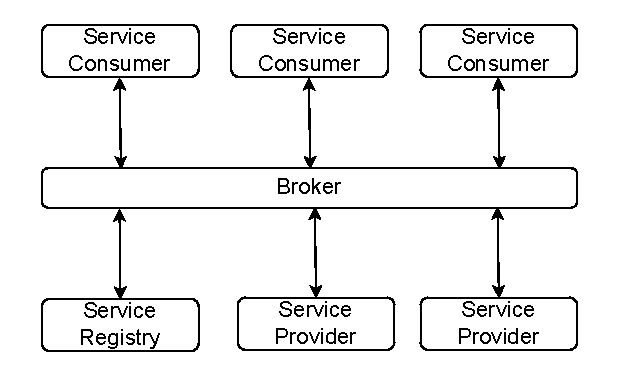
\includegraphics[scale=0.80]{imglib/soa/soa}
    \caption{Aufbau der Service-oriented Architecture}
    \label{fig:soa}
  \end{figure}
\end{frame}

\begin{frame}{Service-oriented Architecture: Beispiel E-Commerce I}
  \begin{itemize}
    \item \texttt{OrderService}: Dienst für Verwaltung von Bestellungen
    \item \texttt{PaymentService}: Dienst verantwortlich für die Abwicklung von Zahlungen
    \item \texttt{ShipmentService}: Dienst zuständig für den Versandprozess
  \end{itemize}
\end{frame}

\begin{frame}{Service-oriented Architecture: Beispiel E-Commerce II}
  \begin{figure}[!h]
    \centering
    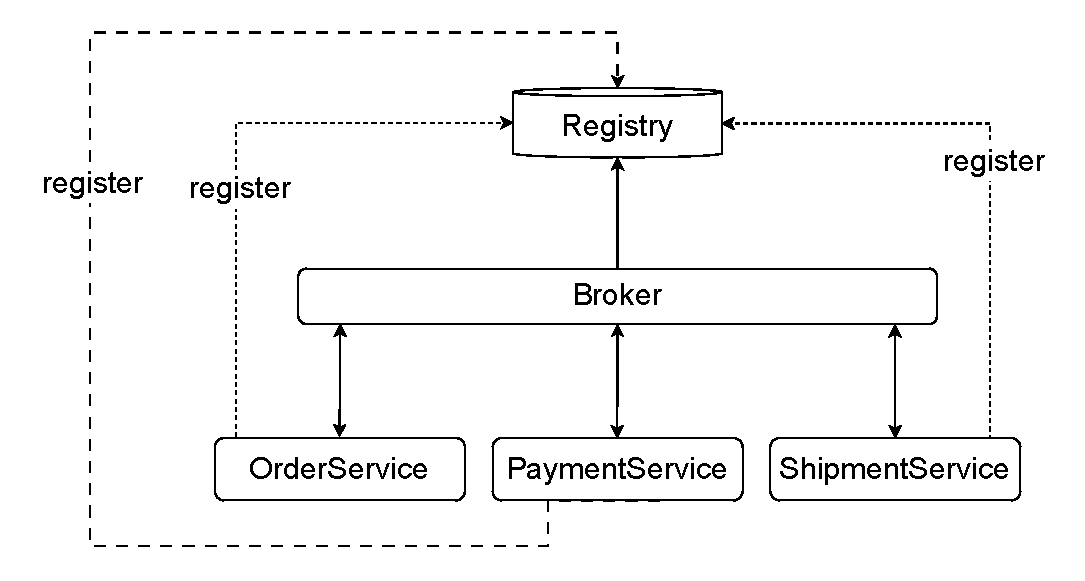
\includegraphics[scale=0.55]{imglib/soa/soa-example}
    \caption{E-Commerce-Beispiel mit Service-oriented Architecture}
    \label{fig:soaecommerce}
  \end{figure}
\end{frame}

\begin{frame}{Service-oriented Architecture: Agilität}
  \begin{itemize}
    \item Lose Kopplung ermöglicht die unabhängige Entwicklung von Services, wodurch Teams autonom arbeiten und die parallele Entwicklung gefördert wird
    \item Dank loser Kopplung und autonomer Teams können Kundenanforderungen schnell umgesetzt werden
    \item Zeit- und Kosteneinsparungen durch die Wiederverwendung von Services
    \item Nachteil: Langfristig könnten sich Abhängigkeiten zwischen den Services entwickeln
    \end{itemize}
\end{frame}
